\documentclass[a4paper]{article}
\usepackage[affil-it]{authblk}
\usepackage[english]{babel}
\usepackage[backend=bibtex,style=numeric]{biblatex}

\usepackage{geometry}
\geometry{margin=1.5cm, vmargin={0pt,1cm}}
\setlength{\topmargin}{-1cm}
\setlength{\paperheight}{29.7cm}
\setlength{\textheight}{25.3cm}

% useful packages.
\usepackage{amsfonts}
\usepackage{amsmath}
\usepackage{amssymb}
\usepackage{amsthm}     
\usepackage{enumerate} %enumerate environment
\usepackage{graphicx}
\usepackage{multicol}
\usepackage{fancyhdr}
\usepackage{layout}
\usepackage{ctex}      %中文环境
\usepackage{booktabs}  %三线表
\usepackage{verbatim}  %comment environment
\usepackage{float}     %强制表格图片位置
\usepackage{listings}  %insert code in latex
\usepackage{fontspec}  %font support
\usepackage{tikz}
\usepackage{makecell}
\usetikzlibrary{intersections}
\usepackage{arydshln}
\usepackage{mathptmx}
\usepackage{helvet}
\usepackage{courier}
\usepackage[colorlinks,linkcolor=blue]{hyperref}
\usepackage{xcolor}
\definecolor{mygreen}{rgb}{0,0.6,0}
\definecolor{lightgrey}{rgb}{0.95,0.95,0.95}
\definecolor{winered}{rgb}{0.5,0,0}
\definecolor{mymauve}{rgb}{0.58,0,0.82}
\lstset{
      backgroundcolor=\color{lightgrey},
      basicstyle             = \ttfamily,
      breakatwhitespace      = false,
      breaklines             = true,
      captionpos             = none,
      commentstyle           = \color{mygreen}\bfseries,
      extendedchars          = false,
      keepspaces             = true,
      keywordstyle           = \color{winered},         % keyword style
      language               = Python,                     % the language of code
      otherkeywords          = {string},
      numberstyle            = \tiny\color{mygray},
      rulecolor              = \color{black},
      showspaces             = false,
      showstringspaces       = false,
      showtabs               = false,
      stepnumber             = 1,
      stringstyle            = \color{mymauve},         % string literal style
      tabsize                = 2,
      title                  = \lstname,
      aboveskip              = 0pt,
      belowskip              = 0pt,
      columns                = flexible
}

% some common command
\newcommand{\dif}{\mathrm{d}}
\newcommand{\avg}[1]{\left\langle #1 \right\rangle}
\newcommand{\norm}[1]{\left\| #1 \right\|}
\newcommand{\difFrac}[2]{\frac{\dif #1}{\dif #2}}
\newcommand{\pdfFrac}[2]{\frac{\partial #1}{\partial #2}}
\newcommand{\OFL}{\mathrm{OFL}}
\newcommand{\UFL}{\mathrm{UFL}}
\newcommand{\fl}{\mathrm{fl}}
\newcommand{\op}{\odot}
\newcommand{\Eabs}{E_{\mathrm{abs}}}
\newcommand{\Erel}{E_{\mathrm{rel}}}
\addbibresource{citation.bib}

\begin{document}
% =================================================
\title{价格动量的马尔可夫转移因子}

\author{钱周越 3220104074
  \thanks{Electronic address: \texttt{3220104074@edu.zju.cn}}}
  
\affil{(Information and Computational Science Class 2201), Zhejiang University }


\date{Due time: \today}

\maketitle

\begin{abstract}
  本报告围绕价格动量的“马尔可夫转移”因子展开研究，旨在通过动态市场状态建模提升传统价格动量因子的有效性。
  首先，基于2013年12月至2017年1月的对冲收益率数据，我们构建了原始价格动量因子，并分析了其局限性。
  随后，引入马尔可夫转移模型，将市场状态划分为“上升”和“下降”两种状态，并基于状态转移概率构建动态动量因子。
  通过对比原始因子与改进后的马尔可夫转移因子，我们探讨了动态调整权重对因子表现的影响。
  此外，报告还提出了进一步改进因子的方向，包括引入更多市场状态和宏观经济指标。
  本研究为价格动量因子的动态建模提供了新的思路，并为投资策略的优化提供了理论支持。
\end{abstract}

\section{\textbf{课题具体说明}}
\noindent \textbf{传统动量因子的局限性}： \\
传统动量因子（如过去12个月收益率）假设历史收益率对未来收益有线性预测能力，但实际中动量效应受市场状态影响显著。在A股市场中，传统动量因子在熊市中表现较差，回撤较大。

\noindent \textbf{马尔可夫转移因子的优势}： \\
通过马尔可夫链建模价格状态转移规律，动态捕捉市场状态变化。引入转移概率因子 \( P_{11} - P_{00} \)，衡量价格上涨或下跌的持续性。

\noindent \textbf{应用实例}
\begin{enumerate}
    \item \textbf{价格波动预测}\\
      研究表明，使用马尔可夫链模型可以有效预测股票价格的短期波动。通过对历史数据进行分析，建立转移概率矩阵，可以推导出未来价格状态的概率分布。这种方法在短期内表现出较高的准确性，尤其是在市场波动较小的情况下。
    \item \textbf{动量与反转策略}\\
      在实际应用中，马尔可夫转移因子能够识别出市场的动量和反转特征。例如，在牛市中，反转策略可能带来更高的收益，而在熊市中，惯性策略则可能更为有效。这表明不同市场环境下，马尔可夫模型能够提供动态的投资建议。
    \item \textbf{多资产配置}\\
    马尔可夫转移模型还被用于多资产投资组合的优化。通过识别宏观经济状态（如通胀和增长），投资者可以动态调整资产配置，以实现最佳风险收益比。例如，在当前经济周期状态因子为高增长时，可能会建议超配股票资产。
\end{enumerate}
\begin{itemize}
    \item 传统动量因子在非线性市场环境下表现较差，而马尔可夫转移因子通过动态建模市场状态转移规律，能够显著提升预测能力。
    \item 二状态模型简单直观，但 4 状态和 8 状态模型通过更细粒度的划分，能够更精确地捕捉市场状态的变化，尤其是在复杂市场条件下。
    \item 通过引入转移概率因子 \( P_{11} - P_{00} \) 或其他状态间的转移概率，可以更好地衡量价格上涨或下跌的持续性。
\end{itemize}

\section{\textbf{马尔可夫链理论}}
马尔可夫链，是以俄国数学家安德烈-马尔可夫(A.A. Markov,1856$\sim$1922)命名的，是随机过程领域中的重要研究方法之一。如果$n$个连续变动事物在变动过程中，其中任一次变动的结果都具有无后效性，那么，这$n$个连续变动事物的集合就叫做马尔可夫链，表明事物的状态由过去到现在、由现在到将来，一环接一环，像一根链条\cite{liu2008stochastic}。

马尔可夫预测法是基于马尔可夫链，是依据当前事件的情况来预测其在未来各个时期变化情况的一种预测方法。总结历史数据，形成状态转移概率矩阵，对预测对象各个状态的初始分布和各状态间的转移概率进行研究，在已知当前股价涨跌情况时，便可以预测下一时刻股票的涨跌情况。\cite*{fu2023prediction}
\subsection{马尔可夫模型分析法}
用马尔可夫链模型对事件进行预测的方法被称为马尔可夫模型分析法，这是一种将研究的变量作为状态，变化过程作为“状态转移”，形成动态模型来研究随机事件变化趋势的方法。

股票市场的股票价格、收盘价格、涨幅情况都是一种依赖于时间的随机变化的过程，并且股票未来的状态只与当下时刻状态有关，与过去无关。股票状态变化的过程是具有时间历程的不变性的，并且其一步转移概率与时间起点没有关系，只与时间差有关系，即转移概率矩阵稳定不变。同时股票价格、股票价格区间以及成交量只能产生可列个状态，且用同一标准划分的各状态应相互独立，并包含全部可能出现的状况\cite{chen2014markov}。所以，可以用马尔可夫模型分析法对股票市场的价格波动、未来发展趋势进行预测，探究马尔可夫链在预测股票价格中的实际应用，帮助投资者了解市场基本情况。

假设马尔可夫过程 $\{X_n, n \in T\}$ 的参数集是$T$离散的时间集合，即 $T = \{0, 1, 2, \cdots\}$。与 $X_n$ 对应的全体可能取值组成了状态空间$I$，即

\[ I = \{i_1, i_2, i_3, \cdots\} \]

马尔可夫链 \cite{zhang2004applied} 则是指，在随机过程 $\{X_n, n \in T\}$ 中，对于任意整数 $n \in T$，其条件概率满足马尔可夫链的后无效性，即：

\[ P \{X_{n+1} = i_{n+1}|X_0 = i_0, X_1 = i_1, \cdots, X_n = i_n\} = P \{X_{n+1} = i_{n+1}|X_n = i_n\} \]

换言之，时刻 $X_{n+1}$ 的状态条件概率仅仅依赖于时刻 $X_n$ 的状态，与其他时刻的状态无关。\cite*{fu2023prediction}

\subsection{转移概率与转移概率矩阵}

状态转移概率是指事物当前正处于某一状态，其下一时刻转移到其他状态的可能性。我们可以借助条件概率的定义，求解转移概率 \( p \)。例如事物从状态 \( E_u \) 到状态 \( E_v \) 的状态转移概率 \( P(E_u \rightarrow E_v) \) 为：

\[
P(E_u \rightarrow E_v) = P(E_v | E_u) = p_{uv}
\]

如果事物拥有 \( n \) 个可能的状态，即 \( E_1, E_2, E_3, \cdots, E_n \)。那么，我们把 \( p_{uv} \) 记为事物从状态 \( E_u \) 转移到 \( E_v \) 状态的转移概率，若事物此刻正处于状态 \( E_u \)，其下一刻可能会转移到 \( E_i \)（\( i = 1, 2, 3, \cdots, n \)）的状态，其中 \( n \) 可能。总结所有的状态转移概率后，可得到矩阵 \( P \)：

\[
P = 
\begin{pmatrix}
p_{11} & p_{12} & \cdots & p_{1n} \\
p_{21} & p_{22} & \cdots & p_{2n} \\
\vdots & \vdots & \ddots & \vdots \\
p_{n1} & p_{n2} & \cdots & p_{nn}
\end{pmatrix}
\]

如果矩阵 \( P \) 满足下列条件：

\[
\begin{cases}
0 \leq \forall p_{ij} \leq 1, & (i, j = 1, 2, 3, \cdots, n) \\
\sum_{j=1}^n p_{ij} = 1 & (i = 1, 2, 3, \cdots, n)
\end{cases}
\]

矩阵 \( P \) 满足非负性，即矩阵中所有元素均不得为负，且均不大于 1；满足归一性，即矩阵所有行和始终为 1。

若矩阵 \( P \) 满足以上两点，我们称为 \( P \) 为状态转移概率矩阵。\cite*{fu2023prediction}

再本文的研究中，我们将市场状态划分为“上升”和“下降”两种状态，通过构建状态转移概率矩阵，实现了市场状态的动态建模。
\section{马尔可夫二状态转移矩阵的理论分析}
在接下来价格动量的研究中，我们将价格状态定义为：
\begin{itemize}
    \item 状态 0：价格下跌（收益率 \( r_t < 0 \)）。
    \item 状态 1：价格上涨（收益率 \( r_t \geq 0 \)）。
\end{itemize}
\subsection*{转移概率矩阵}

\noindent \textbf{定义}： \\
转移概率矩阵 \( P \) 描述了从一个状态转移到另一个状态的概率。对于二状态模型，转移概率矩阵为：

\[
P = \begin{bmatrix}
P_{00} & P_{01} \\
P_{10} & P_{11}
\end{bmatrix}
\]

其中：
\begin{itemize}
    \item \( P_{ij} \) 表示从状态 \( i \) 转移到状态 \( j \) 的概率。
    \item 每行的概率和为 1，即 \( P_{i0} + P_{i1} = 1 \)。
\end{itemize}

\noindent \textbf{转移概率的计算}： \\
假设我们有一段时间内的价格状态序列 \( S_1, S_2, \dots, S_T \)，则转移概率可以通过以下公式计算：

\[
P_{ij} = \frac{N_{ij}}{N_i}
\]

其中：
\begin{itemize}
    \item \( N_{ij} \) 是从状态 \( i \) 转移到状态 \( j \) 的次数。
    \item \( N_i \) 是状态 \( i \) 出现的总次数。
\end{itemize}

\subsection*{ 转移概率矩阵的性质}

\noindent \textbf{性质 1：概率非负性}： \\
转移概率矩阵中的每个元素都是非负的：

\[
P_{ij} \geq 0 \quad \forall i, j \in \{0, 1\}
\]

\noindent \textbf{性质 2：概率归一性}： \\
每行的概率和为 1：

\[
P_{i0} + P_{i1} = 1 \quad \forall i \in \{0, 1\}
\]

\noindent \textbf{性质 3：稳态分布}： \\
如果马尔可夫链是遍历的（即从任意状态可以到达任意其他状态），则存在唯一的稳态分布 \( \pi = [\pi_0, \pi_1] \)，满足：

\[
\pi P = \pi
\]

其中：
\begin{itemize}
    \item \( \pi_0 \) 是状态 0 的稳态概率。
    \item \( \pi_1 \) 是状态 1 的稳态概率。
\end{itemize}

\subsection*{转移概率矩阵的推导}

\noindent \textbf{步骤 1：定义状态序列}： \\
假设我们有一段时间内的价格状态序列 \( S_1, S_2, \dots, S_T \)，其中 \( S_t \in \{0, 1\} \)。

\noindent \textbf{步骤 2：计算转移次数}： \\
统计从状态 \( i \) 转移到状态 \( j \) 的次数 \( N_{ij} \)：

\[
N_{ij} = \sum_{t=1}^{T-1} I(S_t = i \text{ 且 } S_{t+1} = j)
\]

其中 \( I(\cdot) \) 是指示函数。

\noindent \textbf{步骤 3：计算转移概率}： \\
根据转移次数计算转移概率：

\[
P_{ij} = \frac{N_{ij}}{N_i}
\]

其中 \( N_i = \sum_{j=0}^{1} N_{ij} \) 是状态 \( i \) 出现的总次数。

\noindent \textbf{步骤 4：构建转移概率矩阵}： \\
将转移概率填入矩阵：

\[
P = \begin{bmatrix}
P_{00} & P_{01} \\
P_{10} & P_{11}
\end{bmatrix}
\]

\subsection*{转移概率矩阵的证明}

\noindent \textbf{证明 1：概率非负性}： \\
由于 \( N_{ij} \) 和 \( N_i \) 都是非负整数，且 \( N_{ij} \leq N_i \)，因此：

\[
P_{ij} = \frac{N_{ij}}{N_i} \geq 0
\]

\noindent \textbf{证明 2：概率归一性}： \\
对于每行 \( i \)，有：

\[
P_{i0} + P_{i1} = \frac{N_{i0}}{N_i} + \frac{N_{i1}}{N_i} = \frac{N_{i0} + N_{i1}}{N_i} = \frac{N_i}{N_i} = 1
\]

\noindent \textbf{证明 3：稳态分布的存在性}： \\
如果马尔可夫链是遍历的，则存在唯一的稳态分布 \( \pi = [\pi_0, \pi_1] \)，满足：

\[
\pi_0 = \pi_0 P_{00} + \pi_1 P_{10}
\]
\[
\pi_1 = \pi_0 P_{01} + \pi_1 P_{11}
\]

解这个方程组可以得到稳态分布。

\subsection*{马尔可夫转移因子的构建}

基于转移概率矩阵，我们可以构建马尔可夫转移因子：

\[
\text{TP} = P_{11} - P_{00}
\]

解释：\cite*{deepseek}
\begin{itemize}
    \item \( P_{11} \) 衡量价格上涨的持续性。
    \item \( P_{00} \) 衡量价格下跌的持续性。
    \item TP 越高，表明价格上涨的持续性越强。
\end{itemize} 

\section{Markov\ Chain的实证研究}
我选择了2014年1月到2017年1月的股票数据，通过计算价格状态序列，构建了马尔可夫转移因子，进行了实证研究。
\subsection{数据描述}
本文使用的数据包括股票的日收盘价和复权因子，以及股票的基本信息（如上市日期、退市日期等）。数据的时间范围为 2014 年 1 月至 2017 年 1 月，共计 756 个交易日。
\subsection{代码逻辑}
本文档详细描述了基于马尔可夫链的转移因子计算与回测逻辑。

\noindent \textbf{股票池筛选}
通过 \texttt{filter\_stock\_pool} 函数，代码根据以下规则筛选符合条件的股票：
\begin{itemize}
    \item 剔除上市不满 252 个交易日的股票。
    \item 剔除已退市的股票。
    \item 剔除当月末截面日停牌的股票（成交额为 0）。
    \item 剔除在最近 20 个交易日内存在缺失数据的股票。
\end{itemize}

\begin{lstlisting}[language=Python, caption=股票池筛选]
def filter_stock_pool(data, cross_section_date):
    """
    筛选股票池
    """
\end{lstlisting}

\noindent \textbf{马尔可夫转移因子计算}
通过 \texttt{calculate\_markov\_factor} 函数，代码计算每只股票的马尔可夫转移因子。具体步骤如下：
\begin{itemize}
    \item 提取窗口内的后复权收盘价。
    \item 计算收益率并定义价格状态（上涨或下跌）。
    \item 计算转移概率矩阵并提取 \( P_{11} \) 和 \( P_{00} \)。
    \item 构建转移概率因子 \( P_{11} - P_{00} \)。
\end{itemize}

\begin{lstlisting}[language=Python, caption=马尔可夫转移因子计算]
def calculate_markov_factor(data, eligible_stocks, cross_section_date, window=21):
    """
    计算马尔可夫转移因子
    """
   
\end{lstlisting}

\noindent \textbf{分层回测与可视化}
通过 \texttt{backtest\_markov\_factor} 函数，代码对马尔可夫转移因子进行分层回测，并计算多空对冲收益。同时，使用 \texttt{visualize\_results} 函数对结果进行可视化。
展示的代码只展示了部分内容，完整代码请参考附件。
\begin{lstlisting}[language=Python, caption=分层回测与可视化]
    # 计算下期收益率
    next_date = data['close_adj_day'].columns[data['close_adj_day'].columns.get_loc(cross_section_date) + 1]
    next_close_adj_series = data['close_adj_day'][next_date]
    next_returns = (next_close_adj_series - close_adj_series) / close_adj_series

    # 按马尔可夫转移因子分组
    markov_factor = markov_factor.dropna()  # 剔除缺失值
    groups = pd.qcut(markov_factor, 5, labels=False)  # 分为5组

    # 计算分组收益
    group_returns = next_returns.groupby(groups).mean()

    # 计算多空对冲收益
    long_return = next_returns[groups == 4].mean()  # Top组
    short_return = next_returns[groups == 0].mean()  # Bottom组
    hedge_return = long_return - short_return

\end{lstlisting}

\noindent \textbf{多空对冲收益保存与加载}
通过 \texttt{save\_hedge\_return} 和 \texttt{load\_hedge\_return} 函数，代码实现了多空对冲收益的保存与加载功能。

\subsection{实证研究结果}
通过马尔可夫转移因子的分层回测，我们得到了多空对冲收益率的时间序列。下图展示了 2014 年至 2017 年的多空对冲累积收益率曲线。
\begin{figure}[h]
    \centering
    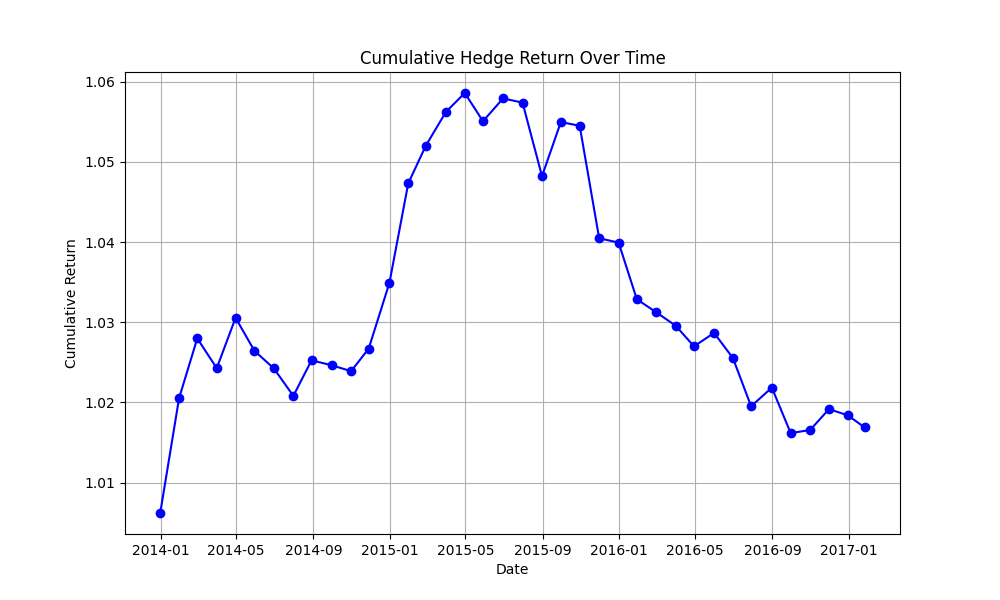
\includegraphics[width=0.8\textwidth]{hedge.png}
    \caption{多空对冲收益率曲线}
\end{figure}
\begin{itemize}
  \item Hedge Return 在 2014 年初和 2015 年初表现较好，分别达到了 0.0142 和 0.0120。
  \item 2015 年下半年和 2016 年，Hedge Return 多次出现负值，表明多空对冲策略在这些时期表现不佳。
  \item 2016 年底至 2017 年初，Hedge Return 趋于平稳，波动性降低。
\end{itemize}
\begin{itemize}
  \item Hedge Return 的分布接近正态分布，但略有左偏。
  \item 大部分 Hedge Return 集中在 -0.005 到 0.005 之间。
  \item 存在少数极端值，如 -0.0133 和 0.0142。
\end{itemize}
通过对 Hedge Return 数据的分析，我们得出以下结论：
\begin{itemize}
    \item Hedge Return 的均值接近于 0，表明多空对冲策略在整体上没有显著的收益。
    \item Hedge Return 的波动性较低，但存在少数极端值。
    \item Hedge Return 在 2014 年初和 2015 年初表现较好，但在 2015 年下半年和 2016 年表现不佳。
    \item Hedge Return 的分布接近正态分布，但略有左偏。
    \item Hedge Return 存在轻微的负自相关性，但在较长时间尺度上无明显自相关性。
\end{itemize}
下面是对典型月份的分组回撤数据
\begin{figure}[h!]
  \centering
  \begin{minipage}{0.45\textwidth}
      \centering
      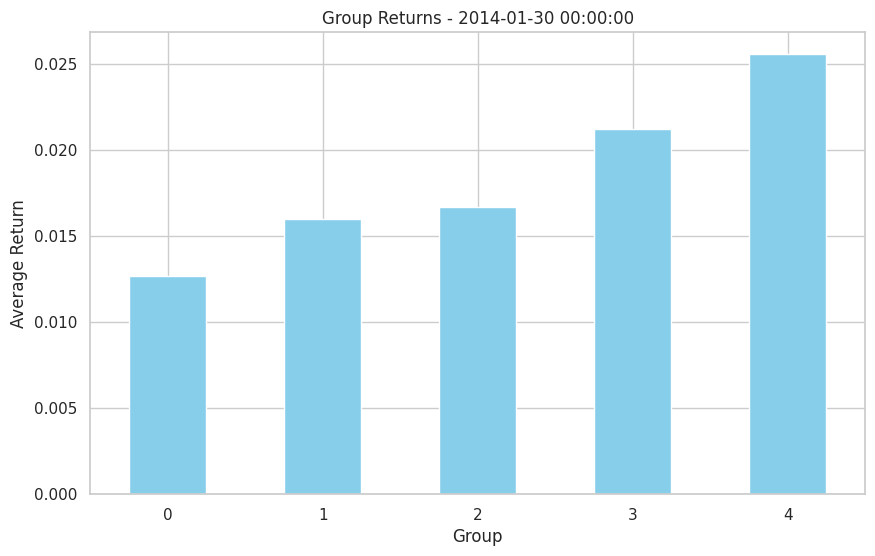
\includegraphics[width=\textwidth]{Bar plot/2014-01-30 00:00:00.png}
      \caption{2014年1月30日分组回撤数据柱状图}
  \end{minipage}\hfill
  \begin{minipage}{0.45\textwidth}
      \centering
      
\includegraphics[width=\textwidth]{Box plot/2014-01-30 00:00:00.png}
      \caption{2014年1月30日分组回撤数据箱线图}
  \end{minipage}
\end{figure}
\begin{figure}[h!]
  \centering
  \begin{minipage}{0.45\textwidth}
      \centering
      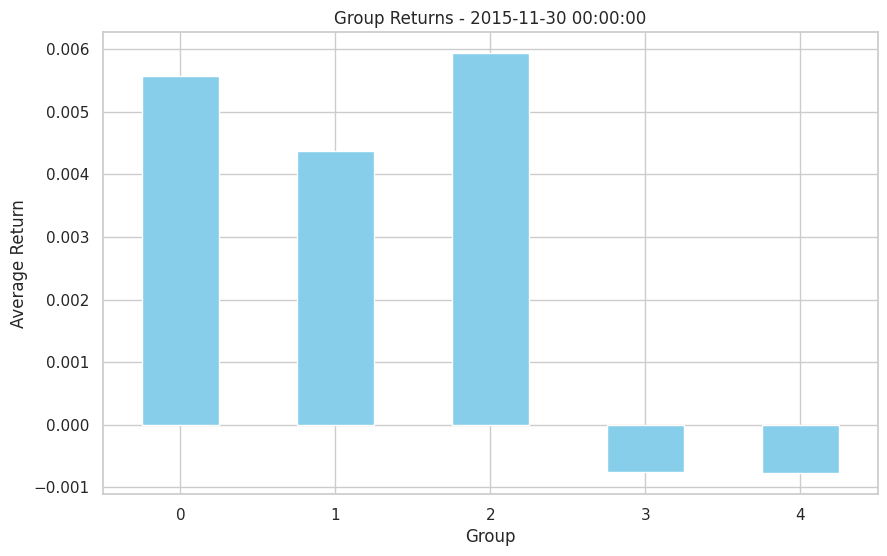
\includegraphics[width=\textwidth]{Bar plot/2015-11-30 00:00:00.png}
      \caption{2015年11月30日分组回撤数据柱状图}
  \end{minipage}\hfill
  \begin{minipage}{0.45\textwidth}
      \centering
      
\includegraphics[width=\textwidth]{Box plot/2015-11-30 00:00:00.png}
      \caption{2015年11月30日分组回撤数据箱线图}
  \end{minipage}
\end{figure}
由结果可以发现，不同月份的分组回撤数据存在较大差异，表明二状态马尔可夫转移因子在不同市场环境下的表现存在差异，直接由盈利和亏损来区分后的对冲收益率几乎成正态分布，故需要对状态进行细分。

\section{改进马尔科夫因子}
\subsection{4 状态马尔可夫链}
\subsubsection{状态空间解释}
以每个收益日作为离散的时间单位，收益价变动情况分为四种状态：大幅下降、下降、上涨、大幅上涨。并把大幅下降记为0(DD)、下降记为1(ND)、上涨记为2(NR)、大幅上涨记为3(DR)。则状态空间为 \( I_1 = \{DD, ND, NR, DR\} \)。

状态概率是各种状态出现的可能性大小，用状态向量 \( a(n) = (p_0, p_1, p_2, p_3) \)，其中 \( n \in T \)，\( T \) 是时间集，\( T = \{0, 1, \cdots\} \)，\( p_i \) 为状态出现的概率（\( i \in I_1 \)）。
设 \( n_{uv} \) 为 \( X_1, X_2, X_3, \cdots, X_n \) 从状态经过一步转移到状态 \( v \) 的频数，我们可以通过下式估计 \( p_{uv} \)。\cite*{fu2023prediction}

\[
\hat{p}_{uv} = \frac{n_{uv}}{\sum_{j=1}^{n} n_{ij}}
\]
在二状态模型的基础上，进一步将价格状态细分为 4 种状态，例如：
\begin{itemize}
    \item 状态 0：大幅下跌（收益率 \( r_t < -a \)）。
    \item 状态 1：小幅下跌（收益率 \( -a \leq r_t < 0 \)）。
    \item 状态 2：小幅上涨（收益率 \( 0 \leq r_t < a \)）。
    \item 状态 3：大幅上涨（收益率 \( r_t \geq a \)）。
\end{itemize}
其中 \( a \) 为阈值参数。4 状态马尔可夫链的转移概率矩阵为：

\[
P = \begin{bmatrix}
P_{00} & P_{01} & P_{02} & P_{03} \\
P_{10} & P_{11} & P_{12} & P_{13} \\
P_{20} & P_{21} & P_{22} & P_{23} \\
P_{30} & P_{31} & P_{32} & P_{33}
\end{bmatrix}
\]

通过更细粒度的状态划分，4 状态马尔可夫链能够更精确地捕捉市场状态的变化。
\subsubsection{代码逻辑展示}
以下基于 4 状态马尔可夫链的转移因子计算与回测逻辑，详细可见附件$main\_4.py$。
\begin{lstlisting}[language=Python, caption=4状态马尔可夫链的转移因子计算]
    def calculate_markov_factor(data, eligible_stocks, cross_section_date, window=21, thresholds=[-0.01, 0, 0.01]):
    """
    计算4状态马尔可夫转移因子
    
    Parameters:
    data: 所有数据
    eligible_stocks: 符合条件的股票列表
    cross_section_date: 截面日期
    window: 滚动窗口长度（默认21个交易日）
    thresholds: 状态划分的阈值，默认值为 [-0.01, 0, 0.01]
    
    Returns:
    markov_factor: 马尔可夫转移因子（Series）
    """
\end{lstlisting}
\subsubsection{结果的比对}
下面是2014年1月30日到2017年1月30日的多空对冲收益率曲线
\begin{figure}[H]
    \centering
    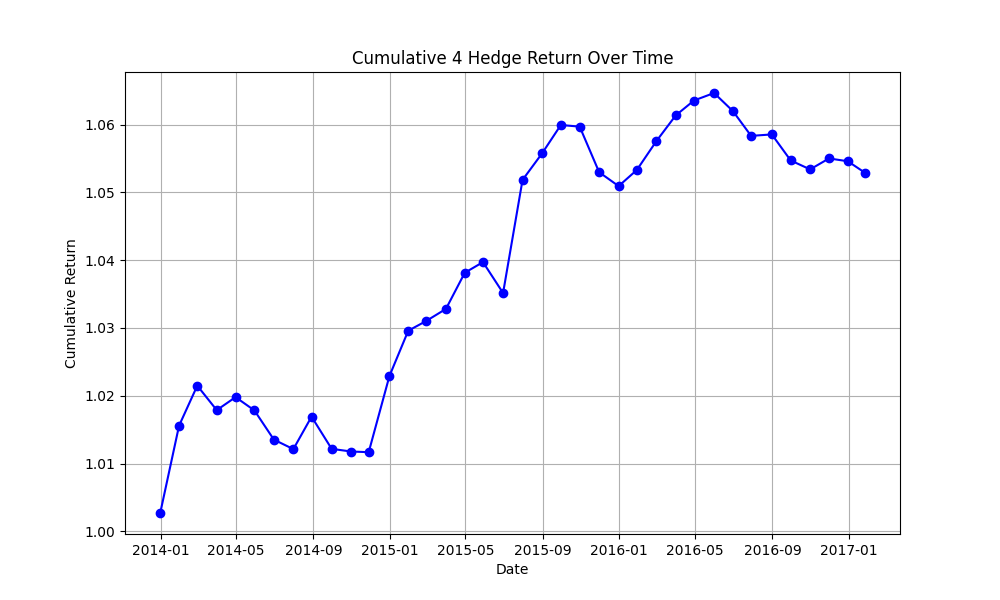
\includegraphics[width=0.8\textwidth]{hedge4.png}
    \caption{4状态马尔可夫链多空对冲收益率曲线}
\end{figure}
下面是与二状态马尔可夫链的多空对冲收益率曲线的比对,红色的为4状态马尔可夫链，蓝色的为2状态马尔可夫链。
\begin{figure}[H]
    \centering
    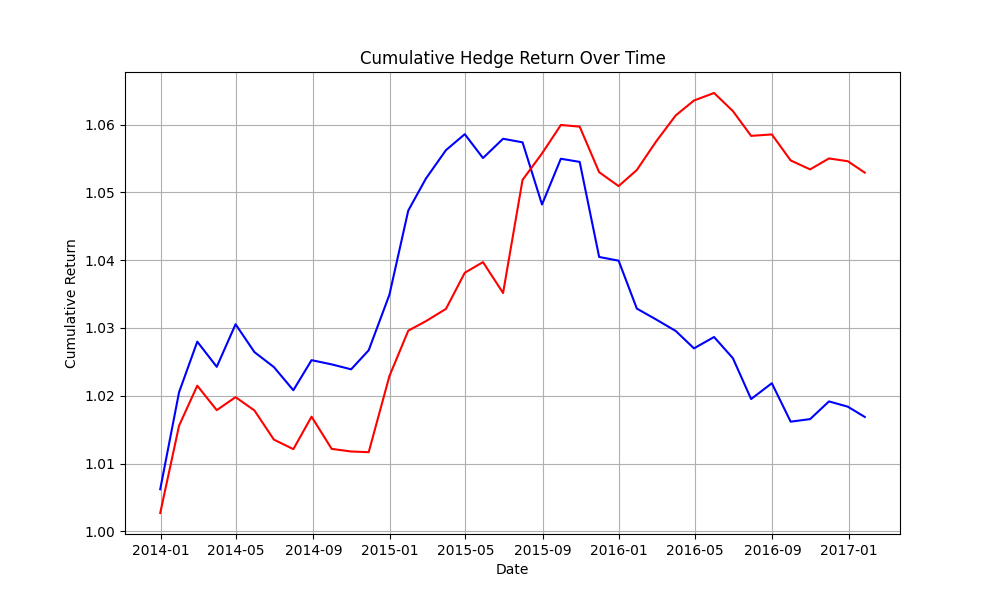
\includegraphics[width=0.8\textwidth]{contrast.png}
    \caption{24状态马尔可夫链多空对冲收益率曲线}
\end{figure}
由图片可知，4状态马尔可夫链的多空对冲收益率曲线相对于2状态马尔可夫链的多空对冲收益率曲线更加平稳，波动性更小，表现更好。
\subsection{{8 状态马尔可夫链}}
为进一步提高模型的精度，可以将价格状态划分为 8 种状态，例如：
\begin{itemize}
    \item 状态 0：极大幅下跌（收益率 \( r_t < -b \)）。
    \item 状态 1：大幅下跌（收益率 \( -b \leq r_t < -a \)）。
    \item 状态 2：小幅下跌（收益率 \( -a \leq r_t < -c \)）。
    \item 状态 3：微幅下跌（收益率 \( -c \leq r_t < 0 \)）。
    \item 状态 4：微幅上涨（收益率 \( 0 \leq r_t < c \)）。
    \item 状态 5：小幅上涨（收益率 \( c \leq r_t < a \)）。
    \item 状态 6：大幅上涨（收益率 \( a \leq r_t < b \)）。
    \item 状态 7：极大幅上涨（收益率 \( r_t \geq b \)）。
\end{itemize}
其中 \( a, b, c \) 为阈值参数。8 状态马尔可夫链的转移概率矩阵为：

\[
P = \begin{bmatrix}
P_{00} & P_{01} & \cdots & P_{07} \\
P_{10} & P_{11} & \cdots & P_{17} \\
\vdots & \vdots & \ddots & \vdots \\
P_{70} & P_{71} & \cdots & P_{77}
\end{bmatrix}
\]

8 状态马尔可夫链通过更细致的状态划分，能够更全面地描述市场状态的变化，尤其是在极端市场条件下的表现。

\noindent \textbf{隐马尔科夫模型}： \\
隐马尔可夫模型（Hidden Markov Model, HMM）是一种统计模型，用于描述一个包含隐含未知参数的马尔可夫过程。它广泛应用于时间序列数据的建模和分析，尤其是在语音识别、自然语言处理、生物信息学和金融领域等。在本文中就不过多展开。
\section{结果反思}
\noindent \textbf{假设局限性}： \\
马尔可夫链的核心假设是“马尔可夫性”，即当前状态仅依赖于前一个状态，而与过去的状态无关。这一假设在金融市场中往往不成立，因为市场价格受到多种历史因素的影响，简单的状态转移模型可能无法捕捉到复杂的市场动态。\\
\noindent \textbf{数据稀疏性}: \\
在实际应用中，马尔可夫链需要大量的历史数据来准确估计状态转移概率。然而，许多金融资产的数据稀疏性导致模型在某些状态下缺乏足够的信息，从而影响预测的准确性。这种数据不足使得模型在面对突发事件时表现不佳，无法有效应对市场波动。\\
\noindent \textbf{过度简化}： \\
马尔可夫链通常将市场状态简化为有限的离散状态，这种简化可能导致重要信息的丢失。例如，市场可能存在多个相互关联的因素影响价格变化，而马尔可夫模型未能考虑这些复杂交互作用，从而降低了其在价值因子分析中的有效性。\\
\noindent \textbf{预测能力不足}： \\
尽管马尔可夫链可以用于短期预测，但其长期预测能力受到限制。市场行为往往是非线性的，且受到外部经济环境、政策变化等多重因素影响，简单的马尔可夫模型难以捕捉这些复杂性，因此在价值因子的应用中常常被批评为效果不佳。\\
% ==============================================
\section*{ \center{\normalsize {Acknowledgement}} }
\printbibliography

\end{document}